\section*{Results}

\subsection*{Shortest path}

On the generated graph with 100 vertices and 500 edges with weights uniformly distributed between 5 and 25 were used Dijkstra's and Bellman-Ford algorithms.

Both algorthms found the same routes as shortest between given vertices. In tablle 1 the results are shown for different size of graphs. 
As it seen from table Dijkstra algorithm has better execution time that is due to it better complexity for sparse graphs. In addition it can be found that
Dijkstra execution time is more sensitive for vertices count change (1-3 rows of table) than Bellman-Ford that is caused by largest term in time complexity $|V|log|V|$ while Bellman-Ford has only linear vertices component $O(|V||E||)$. 
On the other hand Bellman-Ford algorithm is more sensitive for changes in edges count (the time changes more significantly with decreasing and increasing the number of edges).

\begin{table*}[h!]
    \begin{center}
        \begin{tabular}[center]{|c|c|c|c|}
            \hline
            Vertices & Edges & Dijkstra & Bellman-Ford\\
            \hline
            50 & 500 &  0.00018 & 0.00043 \\ \hline
            100 & 500 & 0.00027 & 0.00048 \\ \hline
            150 & 500 & 0.00036 & 0.00056\\ \hline
            100 & 250 & 0.00020 & 0.00028 \\ \hline
            100 & 750 & 0.00032 & 0.00070 \\ \hline         
        \end{tabular}
        \caption{Execution time of algorithm with different graph configuration}    
    \end{center}
\end{table*}

\subsection*{A* algorithm}

In the figure 1 the result of two runs of A* algorithm are shown. Where the red points are points on the path and the grey points are ones which are obstacles.

\begin{center}
    \label{fig:1}
    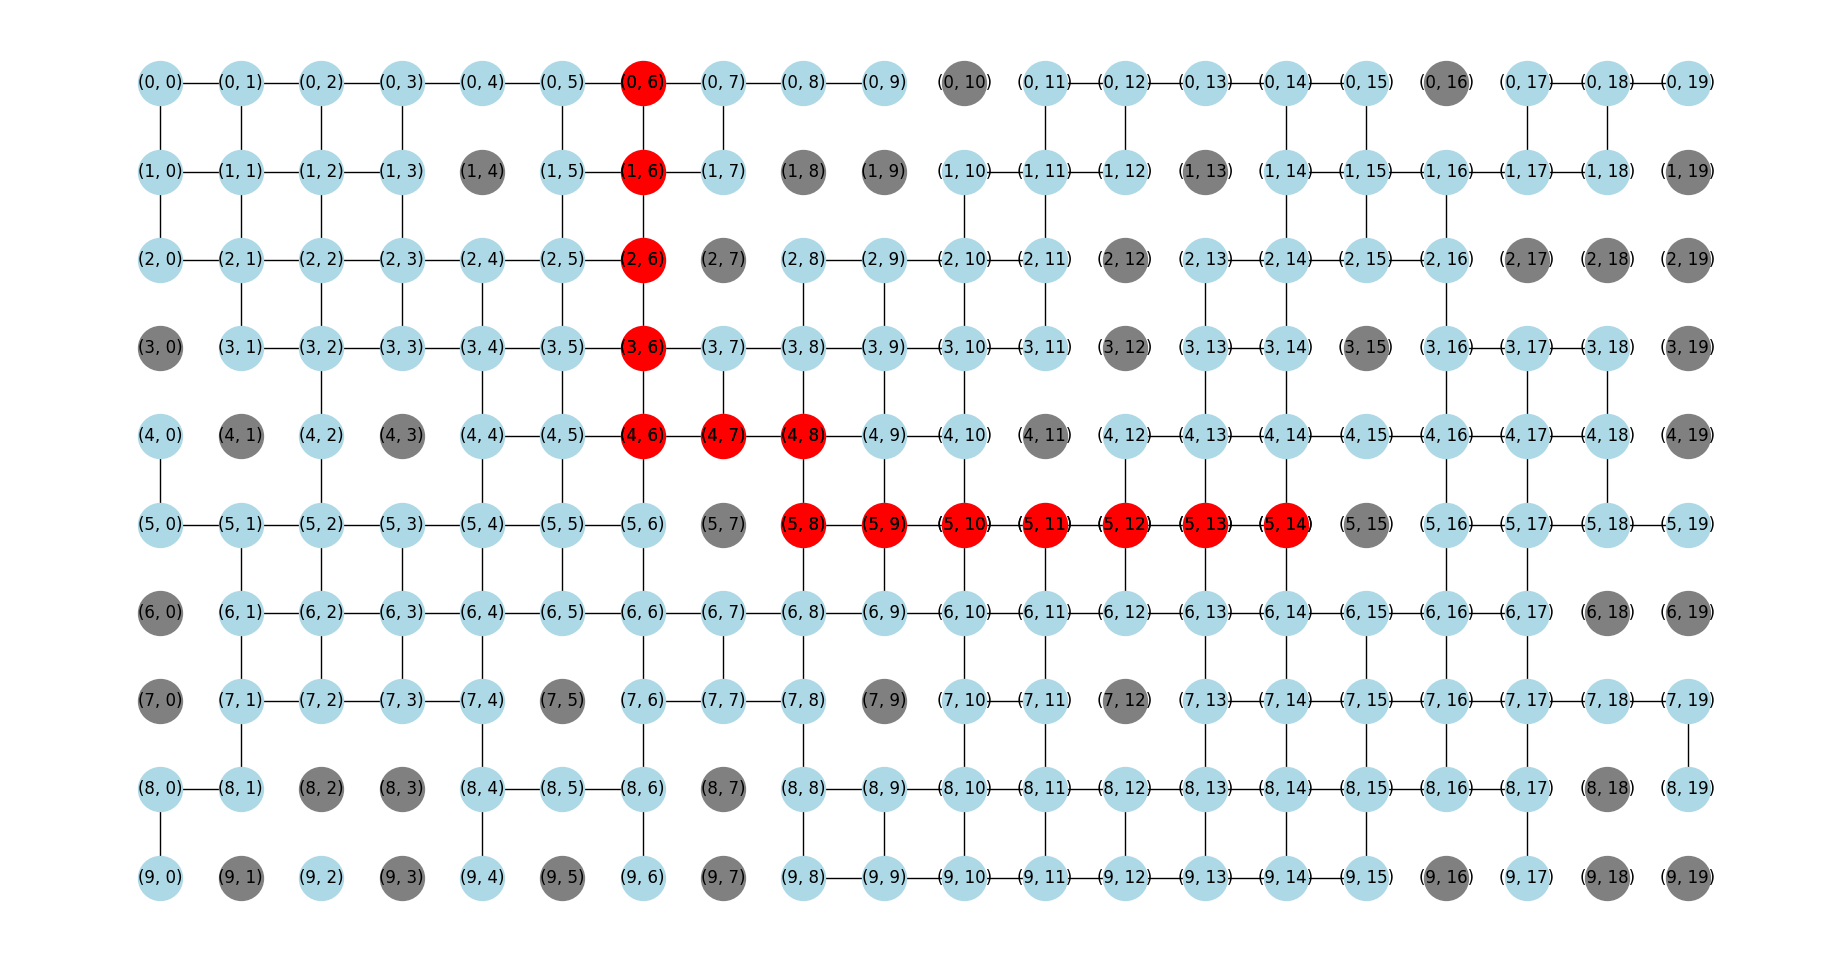
\includegraphics[width=0.75\linewidth]{../results/a_star_1.png}
    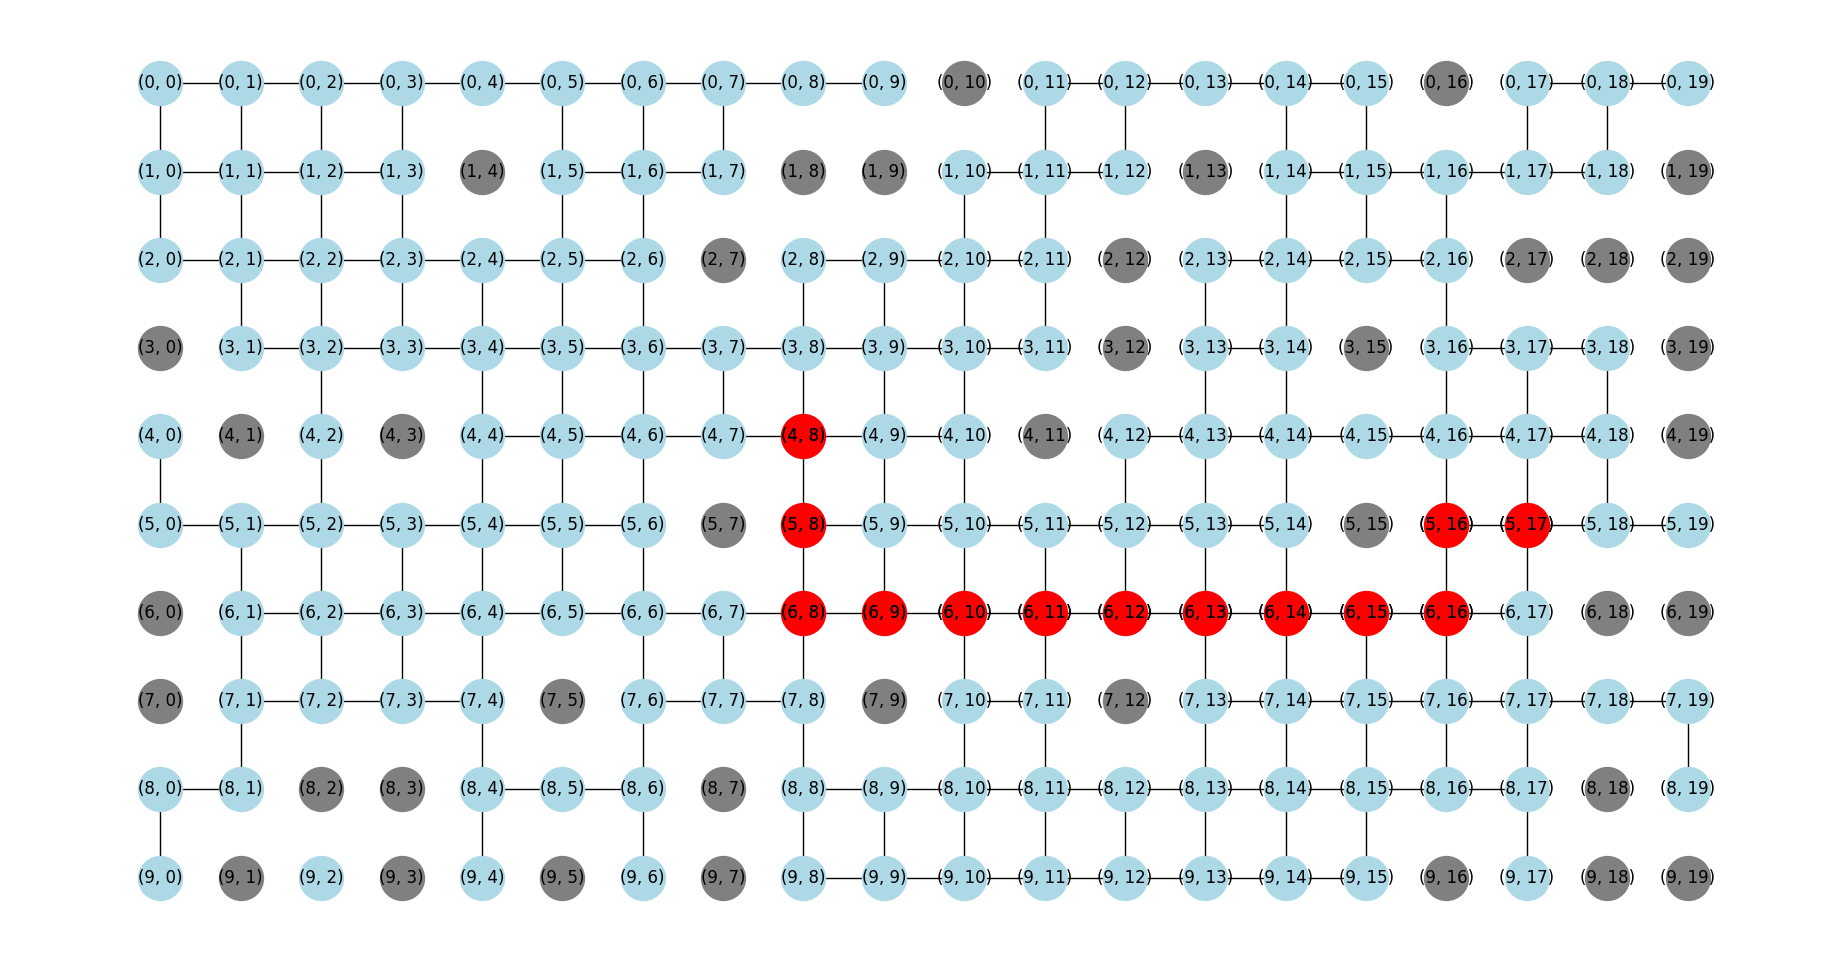
\includegraphics[width=0.75\linewidth]{../results/a_star_2.png}
    \captionof{figure}{Visualization of found path}
\end{center}


\begin{table*}[h!]
    \begin{center}
        \begin{tabular}[center]{|c|c|c|c|c|}
            \hline
            № & From & To & Distant &Time\\
            \hline
            1 & (0, 6) & (5, 14) & 13 & 0.00086 \\ \hline
            2 & (4, 8) & (5, 17) & 12 & 0.00057 \\ \hline
            3 & (6, 12)& (8, 0)  & 14 & 0.00057 \\ \hline
            4 & (6, 1) & (8, 10) & 11 & 0.00034 \\ \hline
            5 & (5, 19)& (5, 0)  & 21 & 0.00059 \\ \hline
            \textbf{Mean: } & & & & \textbf{0.00059} \\  \hline       
        \end{tabular}
        \caption{A* runs on 10x20 grid with 40 obstacles}    
    \end{center}
\end{table*}

\subsection*{Used structures}

In this work mainly was used adjacency list with as it is most commonly used in graphs algorithms due to its conviency of traversing adjacent vertices.
I.e it was used in Dijkstra's and A* algorithm. In Bellman-Ford the edges list representation was used as it allows to implement it in more simple way.